%Receiver
\section{\acl{AODCS}}
\label{recDDadcs}
The \ac{AODCS} of the receiver is basically a scaled down version of the \ac{AODCS} of the emitter, with some scaled down components. Section \ref{ss:recDDads} will thread the attitude determination, section \ref{ss:recDDacs} the attitude control, the orbit determination of the receiver satellites is covered in section \ref{ss:recDDods} and the orbit control in section \ref{ss:recDDocs}. The pointing mechanism for the receiver satellites is significantly more complex compare to the emitter and is described in section \ref{ss:recDDpoint}. Section \ref{ss:recDDoverview} will give an overview of the whole \ac{AODCS} and pointing mechanism of the receiver.
%%%%%%%%%%%%%%%%%%%%%%%%%%%%%%%%%%%%%%%%%%%%%%%%%%%%%%%%%%%%%%%%%%%%%
\subsection{Attitude Determination}
\label{ss:recDDads}
Just as the with the emitter the attitude determination of the receiver satellites is done with sun sensors and a star tracker. The only difference between the two kinds of satellites is that the receiver has got only four sun sensors. In stead of have a sun sensor on each side wall there is only one on the front wall and two on the back looking out at an angle of sixty degrees. This way room is saved and still the entire surrounding of the satellite is covered.

The type of sun sensor and star tracker used are the same as in the emitter satellite. Details can be found in section \ref{ss:emDDads}.

%%%%%%%%%%%%%%%%%%%%%%%%%%%%%%%%%%%%%%%%%%%%%%%%%%%%%%%%%%%%%%%%%%%%%
\subsection{Attitude Control}
\label{ss:recDDacs}
Just as the emitter satellite the receiver uses reaction wheels and magneto torquers for its attitude control. Since the satellite itself is smaller, also the wheels and torquers are scaled down. Figure \ref{fig:catacs} on page \pageref{fig:catacs} shows a possible layout to have control around all axis.

\begin{figure} [h]
\centering
%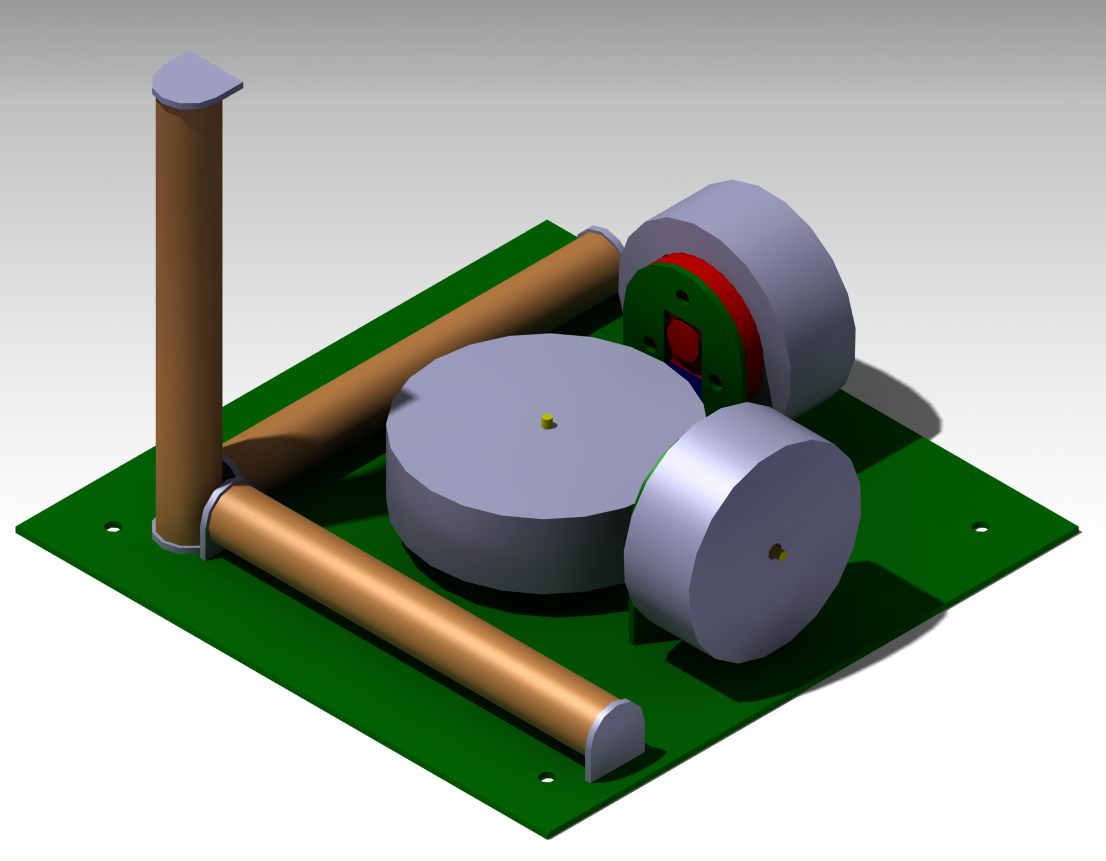
\includegraphics[width=0.8\textwidth]{chapters/img/AC_setup.png}
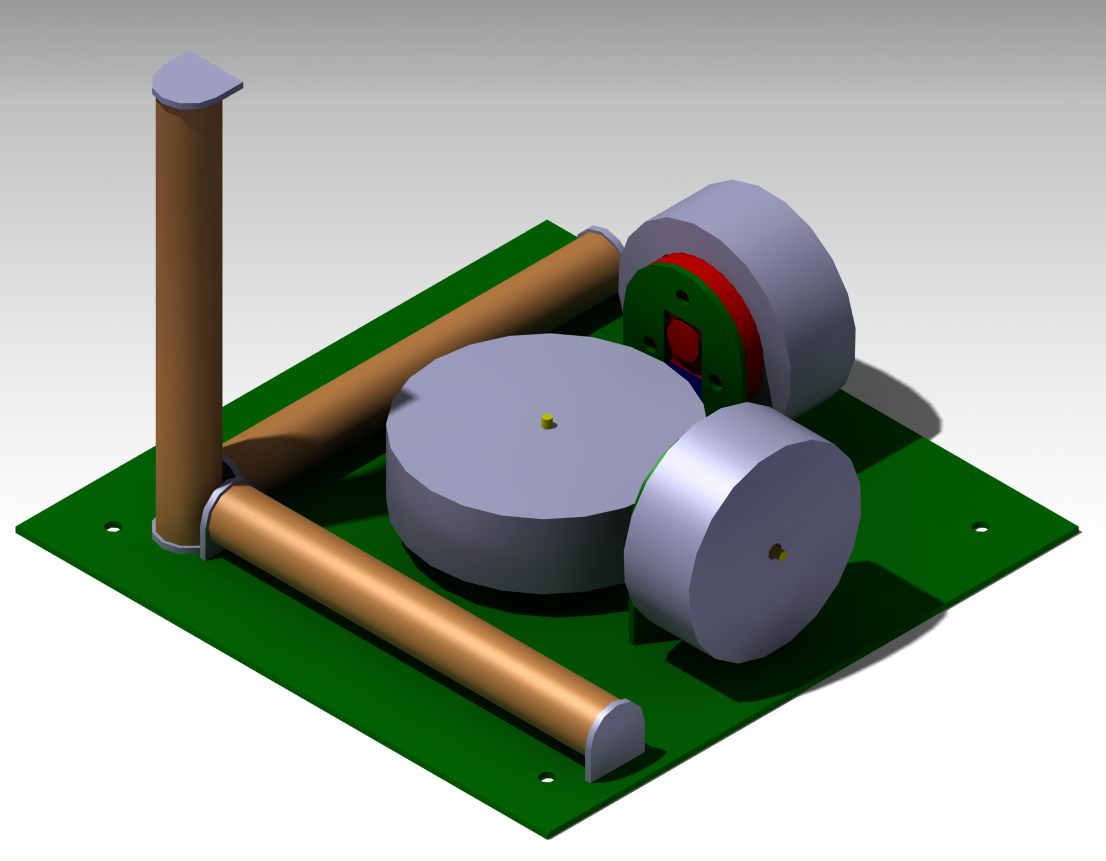
\includegraphics[width=0.8\textwidth, bb=0 0 1106px 861px]{chapters/img/AC_setup.png}
\caption[General layout of the attitude control subsystem]{General layout of the attitude control subsystem with reaction wheels and magneto torquers on all three axis.}
\label{fig:catacs}
\end{figure}

The sizing of the reaction wheels for the receiver satellites is done in the same way as the wheels of the emitter satellite. Filling out equations \ref{distgg} to \ref{distae} for the worst case of the receiver satellites leads to disturbance torques of 

\begin{eqnarray*}
T_g \,=& \frac{3\cdot 398600.4\cdot 10^9}{2\cdot 6878000^3} \left| 1.316 - 0.101 \right| \sin{\left(2\cdot 30^\circ \right)} &= 1.933\cdot 10^{-6}\,Nm\\
T_{sp} =& \frac{1367}{3\cdot 10^8}0.53\left(1+0.6\right)\cos{0^\circ}\left(0.15\right) &= 5.796 \cdot 10^{-7}\,Nm\\
T_m \,=& 4.893\cdot 10^{-5} \cdot 0.1  &= 4.893 \cdot 10^{-6}\,Nm\\
T_a \,=& \dfrac{1}{2} 1.80 \cdot 10^{-12}\cdot 2.2\cdot 0.53 \cdot 7613^2 \left(0.15\right) &= 9.123 \cdot 10^{-6}\,Nm
\end{eqnarray*}

The moments of inertia used are derived from the model of the receiver satellite, i.e. $I_x = 1.307\,kgm^2$,  $I_y = 0.101\,kgm^2$ and $I_z = 1.316\,kgm^2$. Other typical properties are derived using SMAD \cite{larson} and the master thesis of Angel Garza about attitude control of cubesats  \cite{wheelmotor}. The total disturbance torque expected is the sum of the above values $1.65 \cdot 10^{-5}\,Nm$. With a margin of safety of 2 applied this leads to a maximum control torque required of $3.31\cdot 10^{-5}\, Nm$. Taking a angular acceleration of $100 rad/s^2$ ($\sim$ 10\% of maximum) this will lead to a required wheel moment of inertia of $3.306\cdot 10^{-7}\,kgm^2$. With a wheel height $h$ of 1 cm this leads to a wheel skirt thickness $b$ of 1.1 cm. The mass of one wheel is 36 grams.

The magneto torquers chosen are CubeSat Magnetorquers, which are available off the shelf from the cubesat webshop \cite{cubesatshop}. The weight is 30 grams and the diameter is 9 mm and the length is 70 mm. They can provide a torque of 0.2 $Am^2$. Three are required for the 3 axis desaturation. Price is 1150 EUR a piece. Three are needed to desaturate all three wheels.

%%%%%%%%%%%%%%%%%%%%%%%%%%%%%%%%%%%%%%%%%%%%%%%%%%%%%%%%%%%%%%%%%%%%%
\subsection{Orbit Determination}
\label{ss:recDDods}
Just as with the emitter the orbit determination of the receivers is done by the navigation system. For the receiver this is described in section \ref{NaviReceiver}.

%%%%%%%%%%%%%%%%%%%%%%%%%%%%%%%%%%%%%%%%%%%%%%%%%%%%%%%%%%%%%%%%%%%%%
\subsection{Orbit Control}
\label{ss:recDDocs}
For orbit control a $\Delta V$ budget of 165.14 m/s is required (derived in section \ref{frRecDV}).The thruster used for achieving this budget is the M050HP monopropellent thruster from Micro Aerospace Solutions, Inc \cite{h2o2thruster}. It uses hydrogen peroxide ($H_2O_2$) and has a specific impulse $I_{sp}$ of 120 seconds. Using the propellant to dry mass ratio depicted in equation \ref{fuelratio} and using a satellite dry mass of  13.52 kg, a propellent mass of  1.77 kg is needed, this corresponds to 1.23 litres. The thruster has a mass of 6.35 grams. Figure \ref{fig:microthrust} shows the basic thruster layout with the combustion chamber, throat and nozzle.

\begin{figure} [h]
\centering
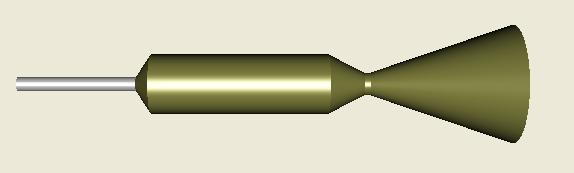
\includegraphics[width=0.8\textwidth]{chapters/img/MAS_acsThruster.jpg}
%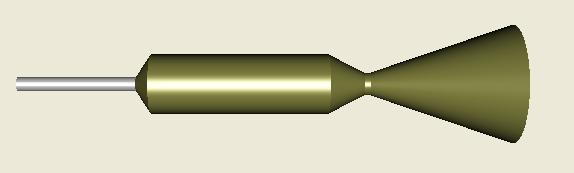
\includegraphics[width=0.8\textwidth, bb=0 0 1106px 861px]{chapters/img/MAS_acsThruster.jpg}
\caption[Micro thruster]{The mono propellent micro thruster from Micro Aerospace Solutions, Inc. \cite{h2o2thruster}}
\label{fig:microthrust}
\end{figure}

%%%%%%%%%%%%%%%%%%%%%%%%%%%%%%%%%%%%%%%%%%%%%%%%%%%%%%%%%%%%%%%%%%%%%
\subsection{Pointing Mechanism}
\label{ss:recDDpoint}
The pointing mechanism is use for pointing the receiver off-nadir towards the ground target. The right ascension difference of $2.18^\circ$ translates into a pointing difference of about $30^\circ$ in both directions. To be able to still make measurements when the distance between the satellites gets bigger a total design pointing angle of $80^\circ$ is chosen, $10^\circ$ extra on both sides. The pointing of the instrument is done by a tumbler, driven by a wheel, connected to a harmonic gear box, attached to a stepper motor. The general layout can be seen in figure \ref{fig:point} on page \pageref{fig:point}. The different parts of the pointing mechanism will be discussed in reverse order in this section.

\begin{figure} [h]
\centering
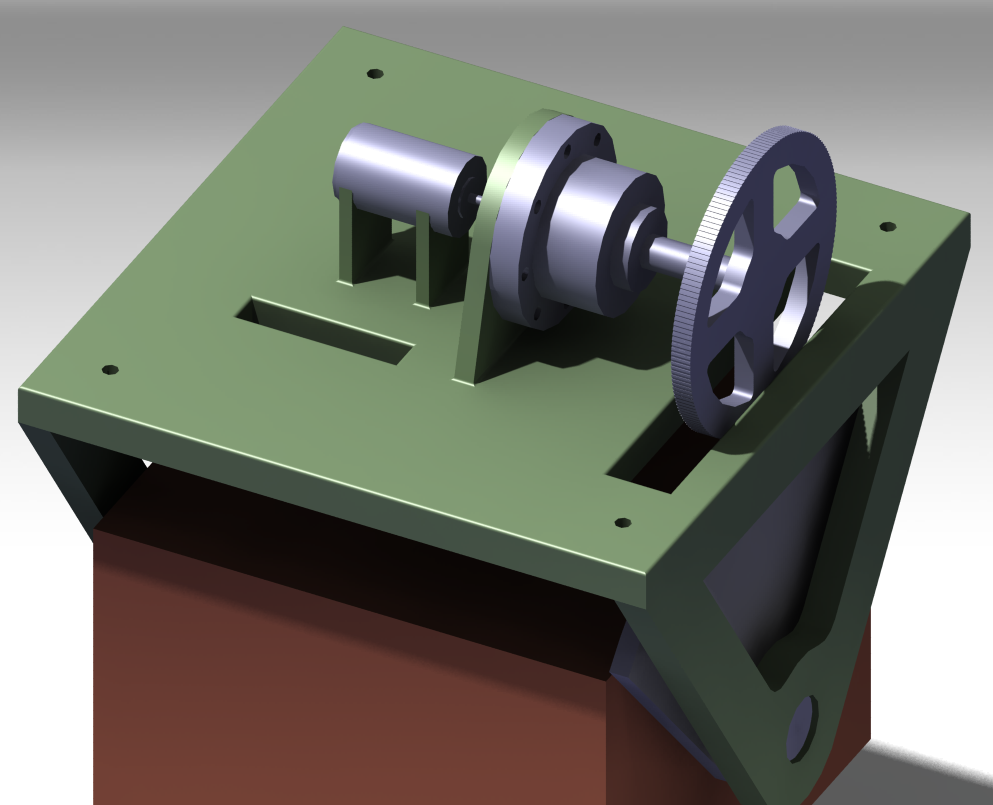
\includegraphics[width=0.8\textwidth]{chapters/img/point_setup.png}
%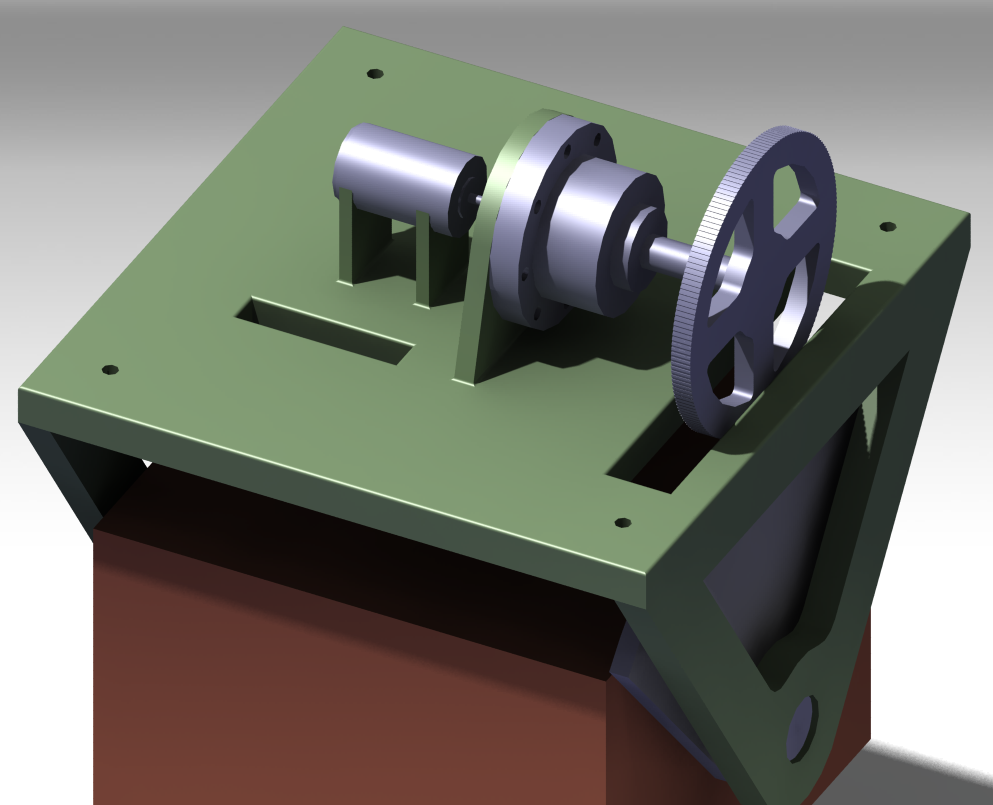
\includegraphics[width=0.8\textwidth, bb=0 0 895px 756px]{chapters/img/point_setup.png}
\caption[General layout of the receiver pointing mechanism]{General layout of the receiver pointing mechanism, with the stepper motor, harmonic drive and the tumbler.}
\label{fig:point}
\end{figure}

The selected stepper motor is a Faulhaber ADM1220. The nominal power is 0.6 Watts. The diameter of the motor is 12 mm, the length of the motor and the axis is 17.4 mm and the motor has a mass of 9 grams. The motor is capable of making 20 discrete steps, giving it a step angle of $18^\circ$. Naturally this is not accurate enough, so a gearbox is needed.

A harmonic drive gearbox is chosen \cite{harmonicdrive}. Generally a harmonic drive gearbox has half the size and one third of the weight of a conventional gear. A Harmonic Drive CSF-8-50 is selected \cite{harmweb}. This gearbox has a gear ratio of 50:1, a diameter of 30 mm, a length of 22.1 mm and a mass of 26 g. With this set-up it is possible to make 20 x 50 = 1000 steps for a full circular rotation of the output axis. Divided over the $80^\circ$ of the possible pointing options this gives a pointing capability with steps of $0.08^\circ$.

The output of the harmonic drive is put into a wheel with the same circumference as the $80^\circ$ sweep of the tumbler, so a complete rotation of the wheel sweeps the receiver from one maximum to the other. This translates into a wheel with a radius of 22.15 mm and a tumbler with a radius of 59.85 mm from the rotation axis of the receiver. The pointing of the receiver can be read by an array of sensors reading a 10-bit ($2^10 = 1024$ steps) grey code from the side of the tumbler. This code is read and digitalised by a set of ten optical link switch.

The along track pointing of the satellite is done by turning the satellite. Since the solar panels are on the sides of the satellite they can still be pointed and the added drag on the satellite is minimal. 
%%%%%%%%%%%%%%%%%%%%%%%%%%%%%%%%%%%%%%%%%%%%%%%%%%%%%%%%%%%%%%%%%%%%%
\subsection{Overview}
\label{ss:recDDoverview}
In table \ref{tab:adcspointbudgetreceiver} on page \pageref{tab:adcspointbudgetreceiver} an overview is given of all masses, costs and power requirements of the parts of \ac{ADCS}, \ac{ODCS} and the pointing mechanism. Because it is essential for the mission that the instrument is pointed towards the ground target extra mass is added to the support structures for the pointing mechanism.
\begin{table}[h]
\begin{tabular}{l | c | c c | c c | c }
Subsystem component    & Number & Mass & Cost & Total mass & Total cost & Power (max)\\ 
                       &   & [g] & [EUR]& [g]  &[EUR] & [W]         \\ \hline \hline
Sun sensors            & 4 & 24  & 11000& 96   & 44000&  0 (0)      \\
Star trackers          & 1 & 375 & 75000& 375  & 75000&  1 (2)      \\ \hline
Reaction wheel motors  & 3 & 8.5 & 176  & 25.5 & 528  &  0.15 (1.5) \\
Reaction wheel disk    & 3 & 36  & 10*  & 108  & 30*  &  0 (0)      \\
Magneto torquers       & 3 & 30  & 1150 & 90   & 3450 &  1 (3)      \\ \hline
Stepper motor          & 1 & 9   & 112  & 9    & 112  &  0.6 (1.2)  \\
Harmonic drive         & 1 & 26  & 180* & 26   & 180* &  0 (0)      \\ 
Tumbler                & 1 & 22  & 10*  & 22   & 10*  &  0 (0)      \\ \hline
Thruster			   & 1 & 15  & 250k & 15   & 250k &  1 (2)      \\
Fuel tanks and pumps   & 1 & 1130 & 300*& 1130  & 300*  & 0 (0)      \\ \hline
Support structures     &	&	 &	    & 1000  & 400* & 0 (0) \\ \hline
Total & & &                             & 2500  & 375k & 3.75 (4.5 rms) \\
&&&&& 435500 FY00\$ &
\end{tabular}
\caption[Mass, cost and power budget of AODCS and pointing mechanism receiver]{Mass, cost and power budget of different parts of the \ac{ADCS}, \ac{ODCS} and pointing mechanism of the receiver. Starred prices are estimations based on material and machining cost.}
\label{tab:adcspointbudgetreceiver}
\end{table}